\section{Introduction}
\label{sec:intro}

\begin{figure}[t]
  \centering
  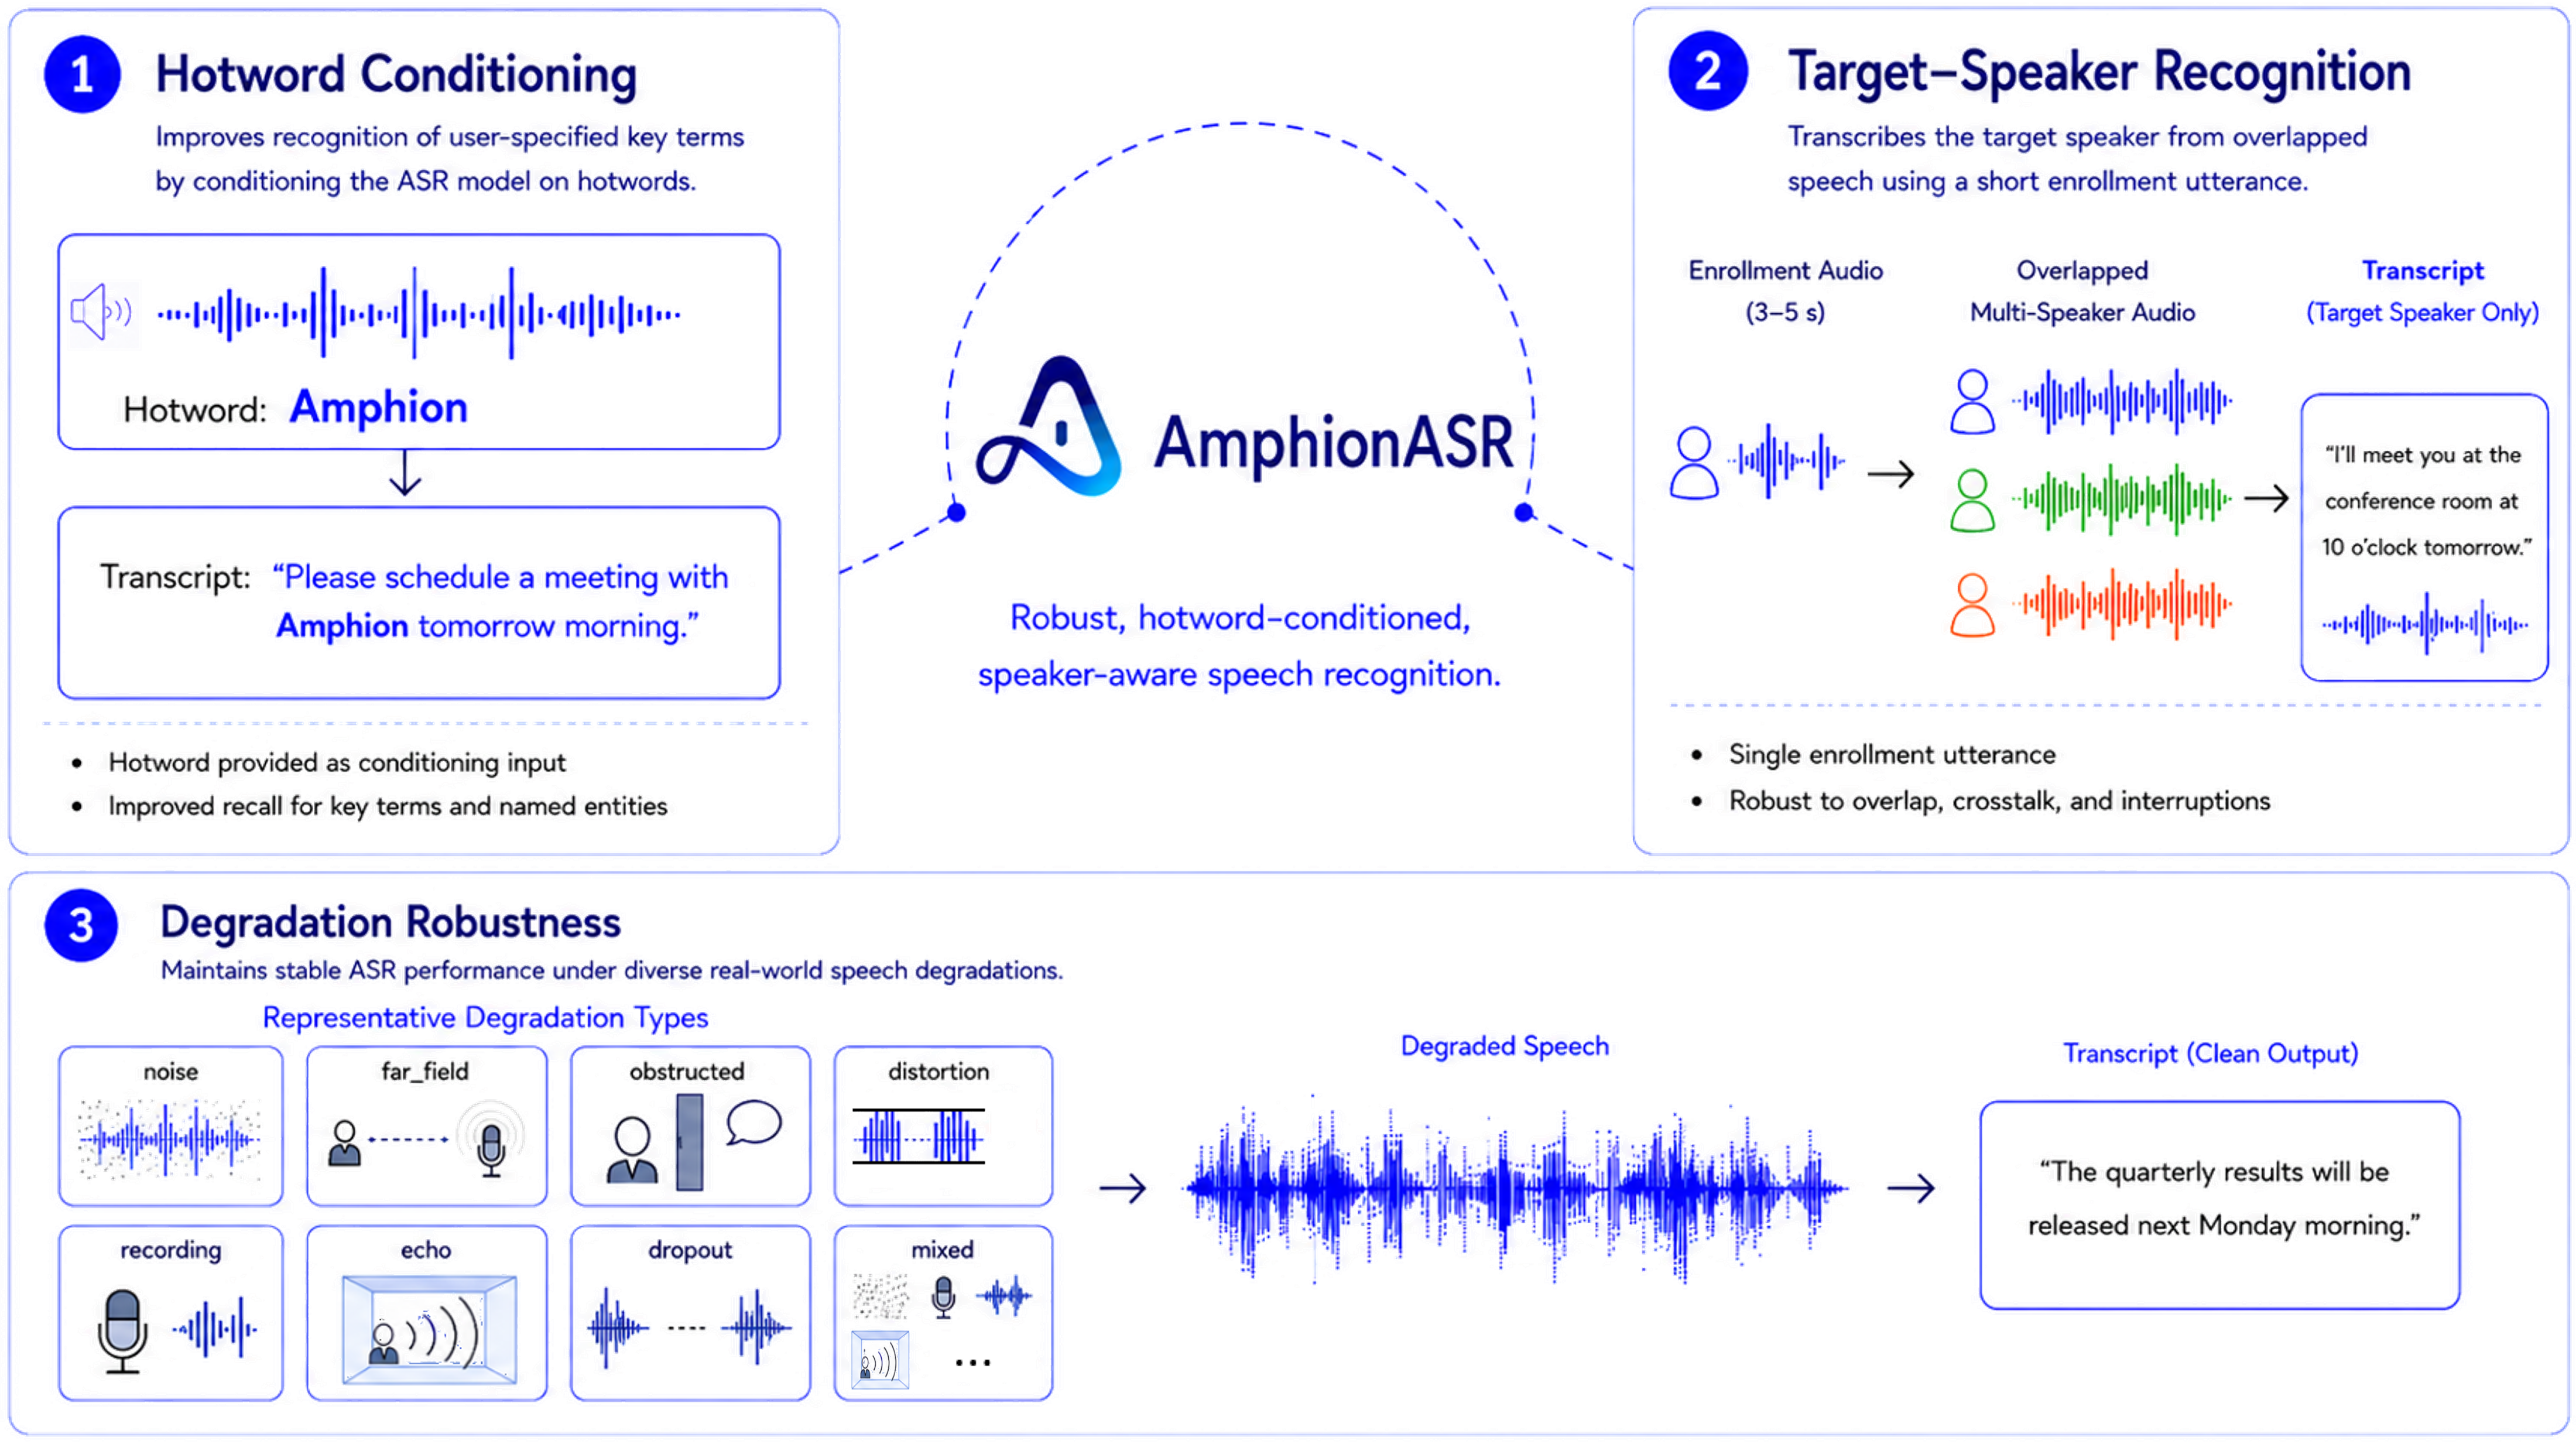
\includegraphics[width=0.92\linewidth]{figures/capabilities-v4.png}
  \caption{Production-oriented capabilities of AmphionASR.
    \emph{Top-left:} hotword conditioning with retrieval-based
    contextual biasing.
    \emph{Top-right:} target-speaker recognition with a $3$--$5$\,s
    enrollment utterance.
    \emph{Bottom:} degradation robustness via SFT on
    Voice-in-the-Wild-2M~\cite{xie2026mega}.
    Whispered-speech ASR is a fourth capability.}
  \label{fig:teaser}
\end{figure}

End-to-end speech recognition has matured from hybrid HMM-DNN systems
\cite{hinton2012deep} to large-scale weakly-supervised models such as
Whisper \cite{radford2023whisper}, while LLM-backed SpeechLLMs
\cite{chu2023qwenaudio,tang2024salmonn,stepaudio22025,kimiaudio2025,qwen2025qwen3asr}
couple strong audio encoders to text decoders within a single
autoregressive model.
We describe \textbf{AmphionASR}, a variant of Qwen3-ASR-1.7B that
addresses four deployment problems---rare entities, overlapping
speakers, real-world degradations, and whispered speech---each tackled
by a dedicated capability described below.

Our contributions are:

\begin{itemize}
  \item \textbf{Hotword conditioning with retrieval-based contextual
        biasing.}
        A pair of small adapters on frozen acoustic and text
        embeddings retrieve top-$K$ hotwords, attaining Recall@$50$
        above $94$\,\% on CommonVoice and improving domain-averaged
        (AVG) entity B-WER on GigaSpeechBench vertical
        domains~\cite{tu2026gigaspeechbench}.
  \item \textbf{Target-speaker recognition with reference audio.}
        On the positive sub-slice of our in-house target-speaker test
        set our model reaches $13.02$\,\% WER, roughly
        $4.1\times$ below the strongest open-source dual-audio baseline
        (Qwen3-Omni, $52.90$\,\%).
  \item \textbf{Degradation-robustness SFT.}
        Joint training on Voice-in-the-Wild-2M yields competitive
        Voice-in-the-Wild-Bench numbers against eight publicly
        reported systems.
  \item \textbf{Whispered-speech ASR.}
        The training recipe includes all $222{,}440$ WhispEar
        training utterances; on the Mandarin wEar test set the model
        reaches $0.58$\,\% CER.
\end{itemize}

Section~\ref{sec:data} documents the training corpus;
Section~\ref{sec:model} introduces the architecture;
Section~\ref{sec:training} details the SFT recipe;
Section~\ref{sec:experiments}--\ref{sec:whisper-asr} report
experiments and capability evaluations;
Section~\ref{sec:analysis} consolidates failure modes;
we discuss limitations in Section~\ref{sec:limitations} and
conclude in Section~\ref{sec:conclusion}.
